\section{Results}
\label{sec:results}

\par
The results from the rig are rather the strength of the rig rather than that of the gears tested. The yellow gears in figure [\ref{im:testRig}] had failed before the loaded white and black gears. The PETG gear was used as the test gear agains the PLA gear. In this configuration the shaft failed as can be seen in figure [\ref{im:rigFailure}]. The results are however still usable.

\par
From the maximum load result of 16.8kg from the second PLA test, it can be calculated that the torque is 16.68Nm [\ref{eq:rig_torque}]. 
\[
    \tau = F \times d
    \]
    \[   
    \tau = 16.8 \times 9.81 \times 0.01 
    \]
    \[
    \tau = 16.68\,\mathrm{Nm}
\]
    

\begin{figure}[H]
    \centering
        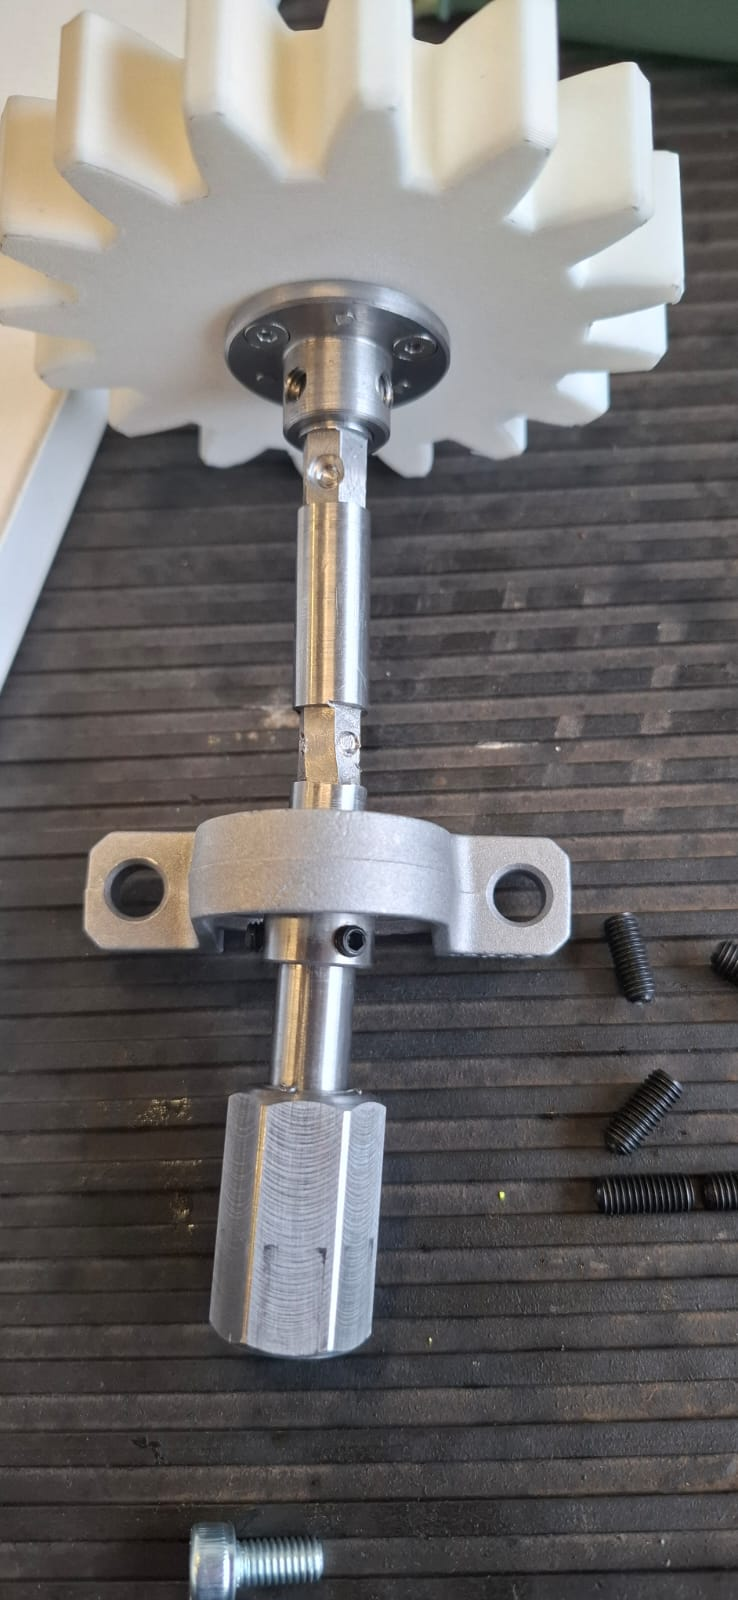
\includegraphics[width=0.5\textwidth]{img/im_rigFailure.jpeg}
        \caption{Rig Failure During Test}
        \label{im:rigFailure}
\end{figure}


\begin{figure}[H]
    \centering
        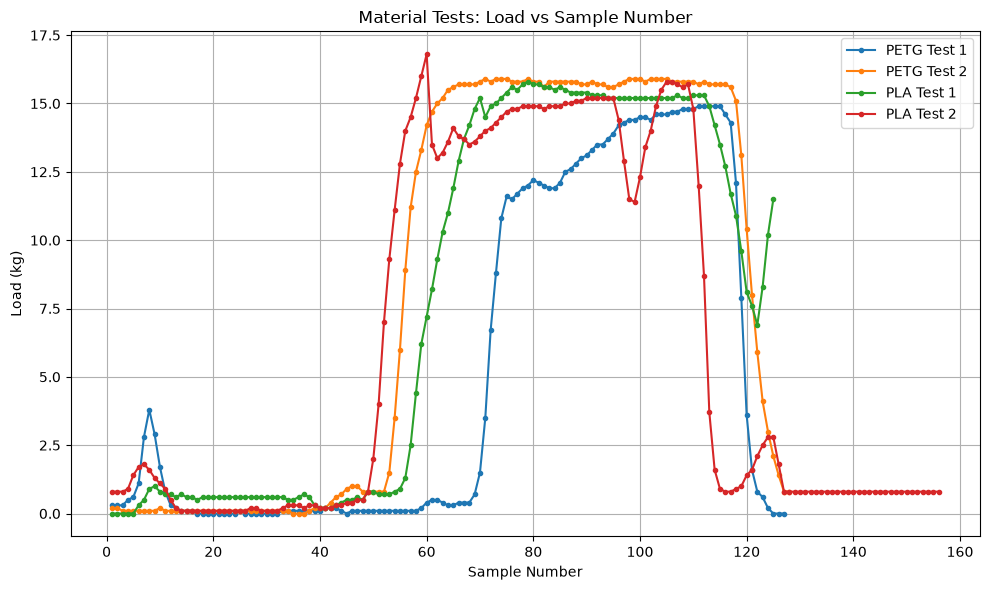
\includegraphics[width=1\textwidth]{figures/chart_loadvssamplenumber.png}
        \caption{Results of the gears tested}
        \label{ch:loadvssamplenumber}
\end{figure}